\newpage


\section{Web Scraping}\label{sec:teoria}

Web Scraping, znany również jako Web Data Extraction, Web Data Scraping, Web Harvesting i Screen scraping, to technika pozyskiwania informacji z zasobów WWW (World Wide Web)\cite{Zhao2017}.
Proces ten, choć niektóre źródła dopuszczają stosowanie metod manualnych\cite{applications-and-tools}, najczęściej wykorzystuje automatyzację za pomocą dedykowanego oprogramowania.
Zautomatyzowanie web scrapingu, z wykorzystaniem takich narzędzi, umożliwia efektywne i szybkie pozyskiwanie ogromnych ilości danych, liczących setki tysięcy, miliony, a nawet miliardy rekordów.

Sieć WWW jest największym źródłem wiedzy i danych w historii ludzkości.
W swoim pierwotnym założeniu została zaprojektowana z myślą o odczycie przez ludzi.
Od momentu powstania gwałtownie się rozrastała i tendencja ta wciąż się utrzymuje (zob. \autoref{fig:statista-data-volume-in-exabytes-per-month}).
Zważając na jej obecnie ogromny wolumen danych, ograniczone zasoby ludzkie pozwalają na przetworzenie jedynie niewielkiego ich ułamka.
Zatem, w obliczu powyższych wyzwań, niezbędna stała się technika web scrapingu polegająca na zbieraniu, ustrukturyzowaniu i przetworzeniu danych, tak aby umożliwić maszynom ich analizę.

\begin{figure}[H]
    \centering
    \captionsetup{width=.8\linewidth}
    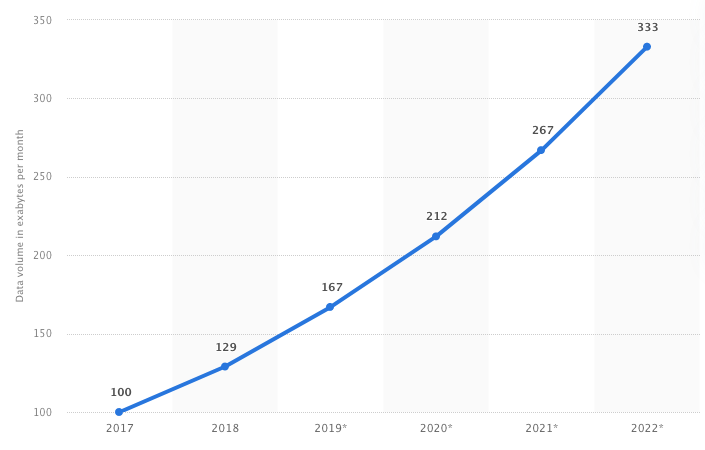
\includegraphics[width=\textwidth]{img/statista-data-volume-in-exabytes-per-month}
    \caption{Wolumen danych w globalnym konsumenckim ruchu IP\newline w latach 2017–2022 (w eksabajtach na miesiąc)\newlineŹródło: \citetitle*{statista-data-volume}~\cite{statista-data-volume}}
    \label{fig:statista-data-volume-in-exabytes-per-month}
\end{figure}

\subsection{Proces Web Scrapingu}\label{subsec:web-scraping-process}

Proces Web Scrapingu, jak przedstawia \autoref{fig:scraping-process}, można podzielić na trzy główne etapy: pobieranie danych, konwersja i przetwarzanie oraz zapis i prezentacja informacji\cite{persson}.

\todo{Popraw ten rysunek}
\begin{figure}[H]
    \centering
    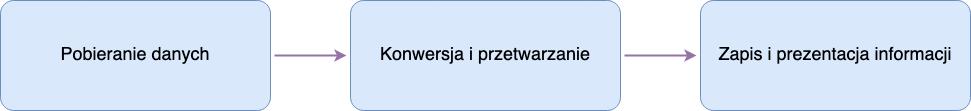
\includegraphics[width=0.8\textwidth]{img/scraping-process}
    \caption{Proces Web Scrapingu}
    \label{fig:scraping-process}
\end{figure}

\subsubsection{Pobieranie danych}

Pierwszy etapem procesu jest pobranie danych zawierających interesujące nas treści.
Zazwyczaj realizuje się to poprzez wysłanie zapytań HTTP (ang. \emph{Hypertext Transfer Protocol}) do jednego lub wielu serwerów WWW\@.
Pobrane, surowe dane zwykle są w formacie HTML (ang. \emph{Hypertext Markup Language}), XML (ang. \emph{Extensible Markup Language}) lub JSON (ang. \emph{JavaScript Object Notation}).

To kluczowy etap z perspektywy cyberbezpieczeństwa, ponieważ to właśnie w nim scraper wchodzi w bezpośrednią interakcję z scrapowaną infrastrukturą.

W związku z zabezpieczeniami stosowanymi przez serwery, ich dostępnością, wydajnością oraz ograniczeniami sieciowymi, etap ten jest zwykle najdłuższym w całym procesie.

\subsubsection{Parsowanie, estrakcja i przetwarzanie danych}

Drugi etap procesu obejmuje operacje przekształcenia wcześniej pobranych danych, takie jak:
\begin{enumerate}
    \item Parsowanie - przekształcenie danych w strukturalną reprezentację łatwiejszą do dalszego przetwarzania
    \item Ekstrakcja - wyodrębnienie interesujących treści
    \item Filtracja - usunięcie niepożądanych i błędnych danych
    \item Mapowanie - przekształcenie danych do pożądanego, jednolitego formatu
\end{enumerate}

\noindent W przypadku scrapowania danych z wielu różnych źródeł, kluczowe jest ich dopasowanie do jednego wspólnego interfejsu, co ułatwia połączenie ich w spójny zbiór danych.

\subsubsection{Zapis i prezentacja informacji}

Ostatni etap Web Scrapingu, obejmujący zapis i prezentację informacji, odgrywa kluczową rolę w udostępnianiu zebranych danych użytkownikom końcowym w przystępnej i zrozumiałej formie\cite{iee-state-of-the-art}.

Dane mogą zostać zapisane w różny sposób, w zależności od potrzeb i preferencji użytkowników docelowych.
Najczęściej stosuje się bazy danych, pliki tekstowe lub arkusze kalkulacyjne, takie jak CSV (ang. \emph{Comma-Separated Values}) czy XLSX (ang. \emph{Microsoft Excel Open XML Spreadsheet}).
Kluczowe jest, aby dane były zapisywane w formatach umożliwiających łatwą przetwarzalność i analizę, co znacznie ułatwia ich dalsze wykorzystanie i analizę\cite{iee-state-of-the-art}.

Prezentacja danych to proces konwersji zebranych informacji na formę wizualną lub tekstową, dostosowaną do łatwego zrozumienia i interpretacji przez użytkowników.
Ten krok może obejmować tworzenie wykresów, tabel, raportów, interfejsów użytkownika oraz innych form wizualizacji, które umożliwiają szybką analizę i wnioskowanie na podstawie dostępnych danych.
Celem jest przedstawienie informacji w klarowny, przystępny sposób, który odpowiada na pytania odbiorców.

\subsection{Wybrane metody Web Scrapingu}\label{subsec:web-scraping-methods}

\subsubsection{Kopiuj-Wklej}

Pierwsza i najbardziej podstawowa metoda web scrapingu to kopiuj-wklej.
Jest to proces manualny, polegający na wybieraniu i kopiowaniu danych bezpośrednio z witryn internetowych, a następnie wklejaniu ich do pliku lub bazy danych.
Metoda ta jest czasochłonna i nieefektywna dla dużych ilości danych, ale może być skuteczna w przypadku małych i prostych zadań\cite{state-of-art}.
Nie wymaga specjalistycznych umiejętności programistycznych, co czyni ją dostępną dla szerszej grupy użytkowników.

\subsubsection{Żądania HTTP i parsowanie HTML}

Kolejną metodą scrapowania jest wykonywanie żądań HTTP w celu uzyskania struktury HTML danej strony internetowej.
Po pobraniu, struktura HTML jest poddawana analizie w celu identyfikacji oraz ekstrakcji żądanych elementów, takich jak tekst, obrazy, hiperłącza i inne.
Często wykorzystuje się specjalistyczne biblioteki programistyczne, które umożliwiają wydobywanie poszczególnych elementów, m.in. poprzez zastosowanie wyrażeń XPath.
Metoda ta jest niezbędna w przypadku stron renderowanych statycznie, kiedy to dostęp do uporządkowanych danych z serwera API jest ograniczony lub niemożliwy.

\subsubsection{Żądania HTTP do serwerów API}

Obecnie, w dobie ogromnej popularności frameworków takich jak Angular oraz bibliotek jak React, duża część aplikacji internetowych jest renderowana dynamicznie.
Aplikacje te komunikują się z zapleczem technicznym (backendem) poprzez API (ang. \emph{Application Programming Interface}) wymieniając dane w uporządkowanej formie np. JSON lub XML.
Fakt ten wykorzystuje kolejna metoda scrapowania polegająca na wykonywaniu żądań bezpośrednio do tych interfejsów z ominięciem warstwy wizualnej aplikacji.
Jest to preferowana metoda, ponieważ znacząco redukuje trudności związane z ekstrakcją danych.
Proces ten jest zwykle szybszy i mniej podatny na błędy, które mogą wynikać ze zmian w strukturze HTML@\.
Należy zauważyć, że struktura HTML ulega częstszym zmianom niż kontakt API, co dodatkowo podkreśla efektywność tej metody w stabilnym pozyskiwaniu danych.

\subsubsection{Wykorzystanie przeglądarki internetowej}

Wśród metod web scrapingu wyróżnia się także tę z wykorzystaniem przeglądarki internetowej.
Podstawę jej działania stanowią biblioteki programistyczne udostępniające wysokopoziomowe API przeglądarek internetowych.
W środowisku JavaScript za przykład posłużyć mogą Puppeteer bazujący na Chrome, Chromium i protokole DevTools
oraz Playwright wspierający silniki Chromium, WebKib i Firefox.
Pierwotnym zastosowaniem wspomnianych wyżej narzędzi było testowanie end-to-end, jednak z czasem rozszerzono ich wykorzystanie i funkcje wspierające web scraping.

Metoda ta sprawdzi się szczególnie w scrapowaniu aplikacji internetowych intensywnie wykorzystujących renderowanie JavaScript
lub kiedy wymagane jest środowisko przeglądarki np. w przypadku zapezpieczenia przez Browser Fingerprinting~\cite{apify-headless-browsers}.
Opisywane biblioteki dysponują rozbudowanym wachlarzem funkcji dających pełną kontrolę nad przeglądarką.
Posiadają klasy takie jak strona, myszka, klawiatura i ekran dotykowy z zachowaniami umożliwiającymi nawigowanie po stronach,
ruchy kursorem i pisanie na klawiaturze.

Ponadto specjaliści w dziedzinie web scrapingu tworzą i rozwijają otwarto-źródłowe rozszerzenia wychodzące na przeciw zabezpieczeniom przeciwko scraperom.
Ukrywają ślad (ang. \emph{fingerprint}) wykorzystanych przeglądarek oraz maksymalnie upodobniają ich zachowanie do człowieka e.g. przez powolniejsze i płyniejsze ruchy kursorem.

To wszystko sprawia, że takie scrapery są relatywnie łatwe do stworzenia.
Natomiast, w związku z wykorzystaniem przez nie rozbudowanego kontekstu przeglądarki, wymagają więcej zasobów i są mniej efektywne.

\subsection{Zastosowania Web Scrapingu}\label{subsec:web-scraping-applications}

Web scraping to jedno z najcenniejszych narzędzi w obszarze pracy z danymi, umożliwiając pozyskanie ogromnych ilości danych z niemal nieograniczonych zasobów internetu\cite{Zhao2017}.
Dzięki automatyzacji i łatwemu dostępowi do niemal nieograniczonych zasobów, metoda ta zapewnia efektywne zbieranie danych przy relatywnie niskich kosztach.
Poniżej opisano przykładowe obszary, w których stosuje się web scraping.

\subsubsection{Business Intelligence}
Web Scraping może służyć za narzędzie, które pomaga firmom w podejmowaniu świadomych decyzji biznesowych i budowaniu przewagi konkurencyjnej.
Najczęściej zbieranymi informacjami są informacje o asortymencie konkurencji, cenach, promocjach, dostępności produktów, opinie klientów oraz dane kontaktowe.
Na rynku istnieją firmy, takie jak Doubledata\cite{doubledata}, które sprzedają web scraping konkurencji w formie usługi.
Podczas przeglądania internetu i literatury, można zauważyć, że rynek e-commerce jest jednym z najczęstszych kontekstów, w którym omawiane jest zastosowanie web scrapingu.

\subsubsection{Marketing i PR}

Web Scraping odgrywa istotną rolę w monitorowaniu treści internetowych i mediów społecznościowych, takich jak Twitter, Facebook, Instagram, LinkedIn czy YouTube.
Jest stosowany do śledzenia opinii publicznej, obserwowania trendów oraz monitorowania wzmianek o marce.
Automatyzacja tego procesu umożliwia szybką reakcję, co jest niezwykle ważne w efektywnym zarządzaniu reputacją marki\cite{monitoring-social-media}.

\subsubsection{Machine Learning i Artificial Intelligence}

Naukowcy i inżynierowie wykorzystują web scraping do pozyskiwania danych, które są niezbędne do trenowania i modeli sztucznej inteligencji\cite{openai-data-collection}.
Dane te wykorzystywane są w różnych celach, od automatycznego rozpoznawania obrazu po analizę języka naturalnego.

\subsection{Scraper}

Web Scraper, w uproszczeniu scraper, to specjalny rodzaj bota przeprowadzający zautomatyzowany proces web scrapingu.

Jak wspomniano w \autoref{subsec:web-scraping-process}, pobieranie danych, czyli etap bezpośredniej interakcji scrapera ze scrapowaną infrastrukturą,
jest jedynym momentem w którym możliwa jest jego identyfikacja i zablokowanie.
Wybrane cechy ruchu sieciowego wykonywanego przez tego typu boty kluczowe w ich detekcji to:

\begin{itemize}
    \item nagłówek \mintinline{text}{User-Agent} wskazuje na narzędzie programistyczne - wget, curl, Postman, Axios itd.
%    \item declares its user-agent as being wget, curl, webcopier etc - it's probably a bot.
    \item nie posiadają nagłówka \mintinline{text}{User-Agent},
%    \item no user-agent (or matching a pattern of known bad ones) - it's probably a bot.
    \item nie posiadają ciasteczek ignorując je,
%    \item no cookie, and wont honor a set cookie - it's probably a bot.
    \item rekurencyjne zapytania o coraz bardziej szczegółowe dane,
%    \item requests details -> details -> details -> details ad nauseum - it's probably a bot.
    \item zapytania jedynie zawartość HTML z ominięciem CSS lub JS,
%    \item requests the html, but not .css, .js or site furniture - it's probably a bot.
    \item duża liczba zapytań HTTP z kodami odpowiedzi > 400.
%    \item generates a large number of HTTP error codes > 400 (1.e 401, 403, 404 \& 500)- it's probably a bot.
    \item pochodzą z mało prawdopodobnego źródła ruchu dla ludzi (np.  Amazon AWS),
%    \item originates from an unlikely human traffic source (i.e Amazon AWS) - it's probably a bot.
    \item nigdy nie posiadają nagłówka z adresem odsyłającym - \mintinline{text}{Referer},
%    \item no referrer, ever - it's probably a bot.
    \item sesje z dużą liczbą zapytań\cite{bot-buster}.
%    \item sessions with a lot of hits. it's probably a bot.
\end{itemize}
